\section{Introduction}
\label{sec:introduction}

\par The goal of this laboratory assignment is to model, dimension, implement and analyse a BandPass FIlter (BPF) circuit with the following specifications:
\begin{enumerate}
	\item Central Frequency: 1kHz;
	\item Gain at Central Frequency: 40dB.
\end{enumerate}

\par It is imposed that to do it we only use at most:
\begin{itemize}
	\item Three $1k\Omega$ Resistors;
	\item Three $10k\Omega$ Resistors;
	\item Three $100k\Omega$ Resistors;
	\item Three $220nF$ Capacitors;
	\item Three $1\mu F$ Capacitors;
\end{itemize}

\par The circuit analised is formed by three voltage sources, $V_{in}$, $V_{CC}$ and $V_{EE}$,
eight resistors, $R_{11}$, $R_{12}$, $R_{2}$, $R_{31}$, $R_{32}$, $R_{33}$, $R_{41}$ and $R_{42}$
three capacitors, $C_1$, $C_{21}$ and $C_{22}$, and one 741 OP-AMP: non-inverting amplifier
with resistive feedback loop. The circuit described
is portrayed in Figure-\ref{fig:circuit}.

\begin{figure}[h] \centering
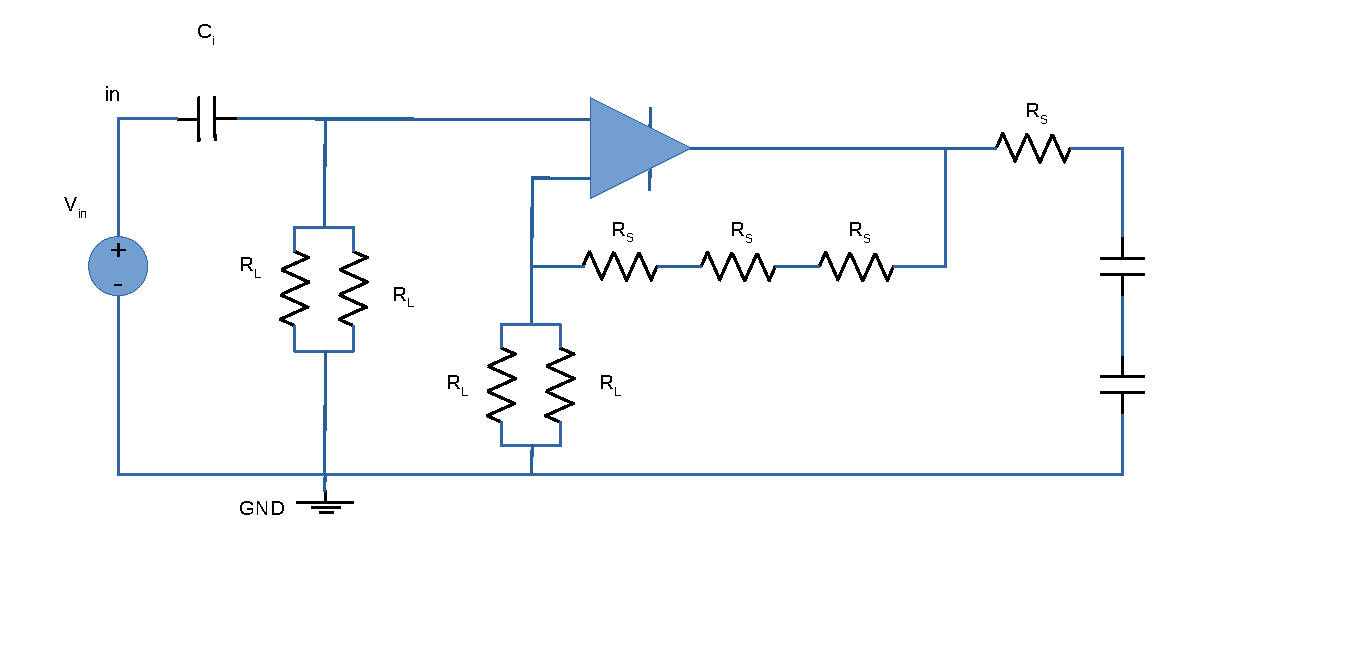
\includegraphics[width=1\linewidth]{circuit.pdf}
\caption{Circuit}
\label{fig:circuit}
\end{figure}


\par Throughout the report it is presented a theoretical analysis, a simulation of the
circuit and its analysis as well as a comparison of the obtained results.

\par In Section~\ref{sec:simulation}, it is executed a simulated analysis of the circuit using
the Ngspice tool to simulate it.
In Section~\ref{sec:analysis}, it is executed a theoretical analysis of the circuit, studying its frequency response, using the Octave maths tool.
In Sectoin~\ref{sec:comparison} both the results obtained in the previous sections are compared side-by-side.
Lastly, in Section~\ref{sec:conclusion}, it is performed a conclusion, bearing in mind the
results from both the theoretical analysis and the simulation, from Section~\ref{sec:analysis}
and Section~\ref{sec:simulation}, respectively.




\newpage
